\documentclass[11pt]{article}
\usepackage[top=0.75in, bottom=0.6in, left=0.75in, right=0.75in]{geometry}
\usepackage{hyperref}
\usepackage{amsmath}
\usepackage{setspace}
\usepackage{booktabs}
\usepackage{graphicx}
\usepackage{float}
\usepackage[numbers]{natbib}
\usepackage{xcolor}

\hypersetup{colorlinks=true, urlcolor=blue!60!black, citecolor=blue!60!black}
\setstretch{1.0}
\setlength{\parindent}{0pt}

\title{\textbf{Positive-Case Count and Synthetic Data Fidelity:\\
A CART-Based Analysis of MIMIC-IV Clinical Data}}
\author{
    William Chen\\
    \textit{University of California, Irvine}\\
    Instructor: Prof.\ Sam Behseta\\
    \textit{DATA298P}\\[4pt]
}
\date{}

\begin{document}
\maketitle

% -------------------------------------------------------
\begin{abstract}
A prior study found that in Bayesian logistic regression the
stabilization threshold is governed not by sample size but by the
number of positive cases for a predictor.
We ask whether the same holds for CART-based synthetic data generation
(\texttt{synthpop}) on MIMIC-IV ($n = 70{,}954$ ICU stays), using two
sweeps that hold the generator fixed and vary only the input: one
varies the rare stratum's positive count $k$ at fixed sample size, the
other varies sample size $n$ at fixed $k$, which together separate
count from prevalence.
Four measurements agree, and none of them follows sample size. Over
matched eight-fold increases, raising $k$ drives divergence from 6--17\%
to exactly zero at $k = 80$ in all six series and cuts interquartile
width by 42--66\%, while raising $n$ moves neither: divergence stays
within a few points of where it started and width changes by $-19$ to
$+10\%$ with no consistent sign. A CART matched to the generator's
control parameters uses the comorbidity in 4--14\% of replicates at every
sample size, against 26--40\% at $k = 250$, and a logistic fit to the same
subsamples detects it in 2--16\% of replicates throughout, with no
consistent gain on real labels over shuffled ones.
The target interactions are small, 0.050 to 0.071 on the logit scale
against a creatinine slope roughly three to four times larger, and a
500-row subsample carries only 6--8\% power to detect them.
The mechanism therefore holds in a narrow sense but does not transfer to
clinical effect sizes.
Two recommendations follow: establish that a target effect is estimable
in the source data before attributing any discrepancy to the generator,
and calibrate variable-selection diagnostics against a permutation null,
whose own rate here moves from 0.00 to 0.32 with class balance alone.
\end{abstract}

% -------------------------------------------------------
\section{Introduction}

Synthetic data is often proposed as a way to share clinical records
without exposing patients, but whether it preserves the relationships
researchers care about is a separate question from whether it looks
realistic overall.
A prior analysis of the \texttt{birthwt} dataset found that under
Bayesian logistic regression, posterior stability depends on the number
of positive cases for a predictor rather than on overall sample size.

This report asks whether the same mechanism holds for CART-based
sequential synthesis. The generator is held fixed throughout; the
question is not which tree-based method performs best but how one of
them behaves when the stratum it must reproduce is small. Because
positive count and prevalence move together whenever sample size is
fixed, a single sweep cannot attribute a change to either, so two
complementary sweeps are run.
Code is available at
\href{https://github.com/ShengPeiWilliam/mimic-synthetic-fidelity}{GitHub Repository}.

% -------------------------------------------------------
\section{Data}

\subsection{Cohort}

MIMIC-IV v2.2 \cite{johnson2023}, restricted to hospital admissions with
an associated ICU stay. One row per ICU stay (73{,}181 stays) was built from
\texttt{icustays}, \texttt{patients}, \texttt{admissions}, and
\texttt{diagnoses\_icd}, the last supplying the comorbidity flags.
Dropping the 3\% of stays with no first-day creatinine leaves 70{,}954
rows; all subsampling draws from this pool.

\subsection{Comorbidity Screening}

Five comorbidities were defined by simplified ICD-9/ICD-10 groupings and
counted by admission rather than by ICU stay, the unit the pool is indexed
on: COPD 7{,}244, CHF 17{,}412, Diabetes 19{,}806, Renal Failure 25{,}369
and Hypertension 34{,}979. The three least common were carried forward.
All five are common in the pool; the rare stratum is created by the
subsampling below, not found in the data.

\subsection{Continuous Variable Selection}

Creatinine was chosen from five first-day lab candidates for its 97\%
coverage and its link to CHF through cardiorenal syndrome. The maximum in
the first 24 hours was taken, capped at the 99.5th percentile ($11$~mg/dL).

% -------------------------------------------------------
\section{Methods}

\subsection{Experimental Design}
\label{sec:design}

Both sweeps draw stratified subsamples, synthesize each with
\texttt{synthpop::syn()} \cite{nowok2016}, and fit
\[
\texttt{hospital\_expire\_flag} \sim \texttt{age} + \texttt{creatinine} + \texttt{comorbidity} + \texttt{comorbidity}{:}\texttt{creatinine}
\]
to both the real subsample and the synthetic table, giving paired
estimates $\hat\beta_{\text{real}}$ and $\hat\beta_{\text{syn}}$ of the
interaction, at $M = 100$ Monte Carlo replicates per grid point.

\begin{center}
\begin{tabular}{llll}
\toprule
Experiment & Held fixed & Varied & What moves \\
\midrule
1. Count sweep    & $n = 500$ & $k \in \{5, 10, 20, 40, 80, 150, 250\}$
                  & count and prevalence together \\
2. Size sweep     & $k = 20$  & $n \in \{250, 500, 1000, 2000, 4000\}$
                  & prevalence only, 8\% to 0.5\% \\
\bottomrule
\end{tabular}
\end{center}

\subsection{Analyses}

We conduct three analyses. (1) A full-pool fit of the interaction supplies
the reference every subsample estimate is read against. (2) The two sweeps
compare $\hat\beta_{\text{real}}$ against $\hat\beta_{\text{syn}}$ at each
grid point on the median and interquartile width of the converged
estimates, with the divergence and inestimable rates kept separate;
Section~\ref{sec:failure} defines the two ways a fit fails. (3) A tree
diagnosis refits the subsamples both sweeps draw with \texttt{rpart} under
\texttt{synthpop::syn.cart}'s control parameters and records whether the
comorbidity earns a split, against a likelihood-ratio test on the same
rows that drops the comorbidity and its interaction together, so both are
asked the same question. Every configuration is re-run with the
comorbidity column shuffled, which leaves the positive count intact and
destroys its association with the outcome, supplying the null.

% -------------------------------------------------------
\section{The Full-Pool Reference}

MIMIC-IV carries no known ground truth, so the interaction fit on the
whole pool stands in as the reference, $\hat\beta_{\text{full}}$, and every
subsample estimate below is read against it. The three interactions differ
in sign, CHF and Diabetes dampening creatinine's main effect while COPD
steepens it, and all three are roughly three to four times smaller than
that main effect.

\begin{table}[H]
\centering
\begin{tabular}{lrrrr}
\toprule
Comorbidity & Creatinine & $\hat\beta_{\text{full}}$ & SE & $p$ \\
\midrule
CHF      & 0.208 & $-0.0497$ & 0.0128 & $1.1\times10^{-4}$ \\
Diabetes & 0.234 & $-0.0709$ & 0.0126 & $2.0\times10^{-8}$ \\
COPD     & 0.188 & $+0.0668$ & 0.0197 & $6.9\times10^{-4}$ \\
\bottomrule
\end{tabular}
\caption{Comorbidity--creatinine interaction on the full pool, with the
creatinine slope it modulates.}
\label{tab:power}
\end{table}

% -------------------------------------------------------
\section{Estimation Failure}
\label{sec:failure}

\subsection{Two Failure Modes}

Fits at the smallest counts failed often enough to matter, and the
failures turned out to be of two distinct kinds. We report their rates as
a result rather than a filtering step: whether an estimate can be produced
at all separates the two levers more sharply than the spread of those that
succeed. Every quantile that follows is computed on converged fits only.

A fit is \textbf{inestimable} when the table holds no positives and the
interaction term comes back as \texttt{NA}; \textbf{divergent} when the
term is estimated but runs past $|2|$, marking a likelihood maximized at
the boundary \cite{heinze2002} rather than a real effect. Only divergence
appears in the real arm, which is built to hold exactly $k$ positives; the
synthetic table generates its own column and can produce none.

The cutoff follows the scale of the target, around $0.05$ in the full
pool, and recomputing at 5 and 10 leaves every comparison pointing the
same way.
Both modes are reported as shares of all $M$ replicates, so converged,
inestimable and divergent sum to one.

\subsection{Failure Under Each Lever}

\begin{figure}[H]
    \centering
    \begin{minipage}{0.47\textwidth}
        \centering
        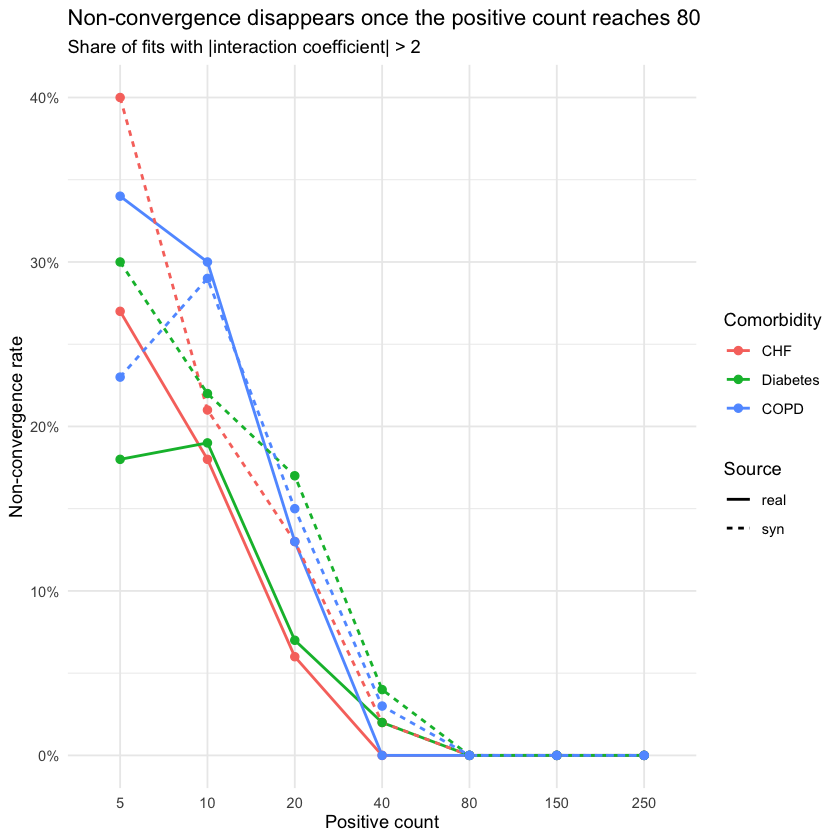
\includegraphics[width=\textwidth]{../figures/nonconvergence.png}
    \end{minipage}
    \hfill
    \begin{minipage}{0.47\textwidth}
        \centering
        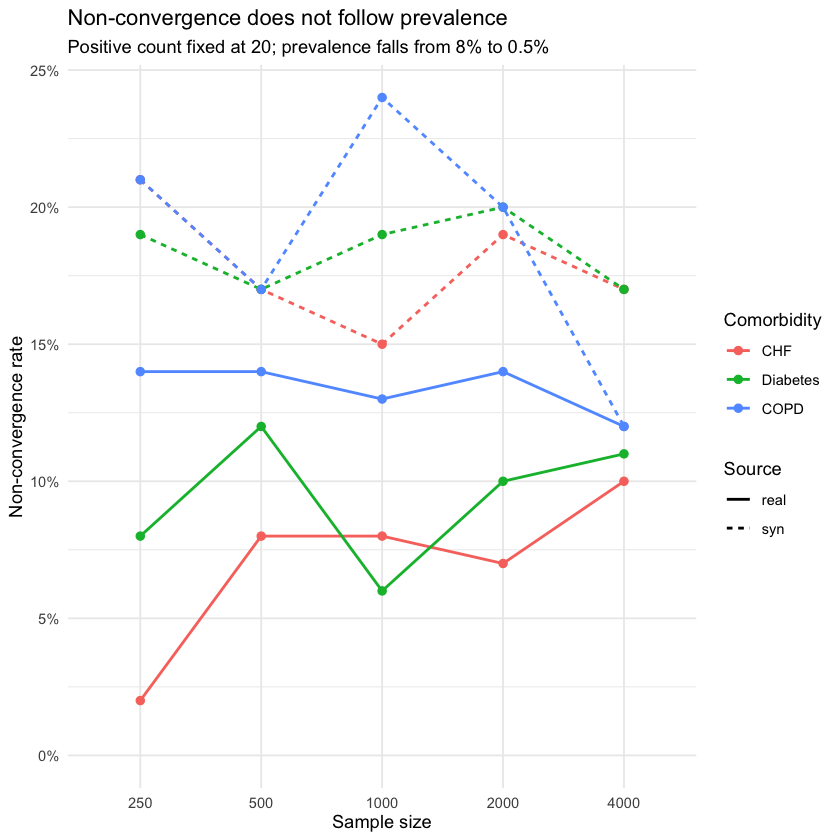
\includegraphics[width=\textwidth]{../figures/size_divergence.png}
    \end{minipage}
    \caption{Divergence rate under each lever, three comorbidities
    $\times$ two sources in both panels. Left: positive count varying at
    $n = 500$. Right: sample size varying at $k = 20$, where prevalence
    falls from 8\% to 0.5\%. Inestimable fits occur on the synthetic side only and are reported in the text.}
    \label{fig:nonconv}
\end{figure}

\paragraph{Count sweep.}
All six curves reach zero at $k = 80$ and stay there. The threshold moves
with neither prevalence, which varies nearly threefold across the three
comorbidities, nor the sign of the interaction. Below it, divergence runs
at 18--40\% at $k = 5$ and is higher on the synthetic side in ten of the
twelve failing cells. The inestimable rate is narrower still: synthetic only,
$k = 5$ only, at 4--6\%.

\paragraph{Size sweep.}
No sample size does the same. Over the matched 8-fold increase in $n$
every series changes by between $-29\%$ and $+25\%$, and none comes near
zero (Figure~\ref{fig:nonconv}, right). COPD is the plainest case: its
real arm fails at 12--14\% at every one of the five sample sizes.
The inestimable rate is zero in all fifteen cells, including at $n = 2000$,
where prevalence matches the $k = 5$ cells that lost the stratum 4--6\% of
the time. Failure follows the count, and only the count.

% -------------------------------------------------------
\section{Results}

\subsection{Experiment 1: Count Sweep}

Spread narrows steadily with the count: from $k = 20$ to $k = 250$ every
one of the six series loses 55\% to 69\% of its width, and none has
flattened by the end of the range. It is still not enough. Even the
narrowest cell, the CHF real arm at $k = 250$, has an interquartile width
of 0.194 against its reference of 0.0497 (Table~\ref{tab:power}), nearly
four times the quantity being estimated. The low end of the span rests on
fewer replicates, 6\% to 44\% being discarded below $k = 40$, but all of
them for diverging, so the decline is if anything understated.

\begin{figure}[H]
    \centering
    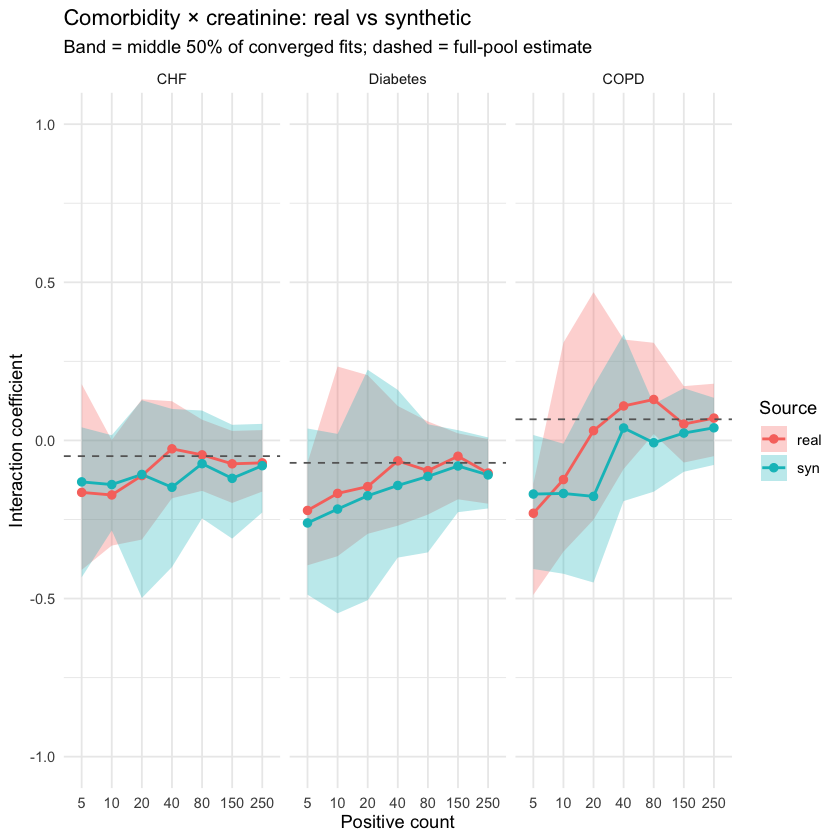
\includegraphics[width=0.55\textwidth]{../figures/spread_ribbon.png}
    \caption{Comorbidity $\times$ creatinine, real vs.\ synthetic. Band =
    middle 50\% of converged fits, dashed line = $\hat\beta_{\text{full}}$.}
    \label{fig:spread}
\end{figure}

What low counts cost is precision, not location: in 39 of the 42 cells the
middle half of the estimates still contains $\hat\beta_{\text{full}}$, the
three exceptions all COPD at $k \leq 10$. The two arms differ on both
counts, and in the same direction. The synthetic median sits below the
real one in 17 of the 21 counts, and where neither side fails at all
($k \geq 80$) synthetic widths run 1.1 to 1.6 times the real ones for CHF
and Diabetes and roughly equal for COPD.

\subsection{Experiment 2: Size Sweep}

The narrowing Experiment 1 found does not reappear under the other lever.
Over roughly eightfold increases in each, $k$ from 20 to 150 and $n$ from
500 to 4000, the count cuts width by 42\% to 66\% in all six series while
the sample size changes it by between $-19\%$ and $+10\%$ with no
consistent sign (Figure~\ref{fig:size}). Across the full sixteen-fold
range of $n$ the widths never leave the band Experiment 1 recorded at
$k = 20$.

The count was held at 20, the last configuration in which it still binds:
failure there runs 6--17\% of replicates against 0--4\% at $k = 40$ and none
from $k = 80$ up. If sample size can substitute for count, this is where
it would show.

\begin{figure}[H]
    \centering
    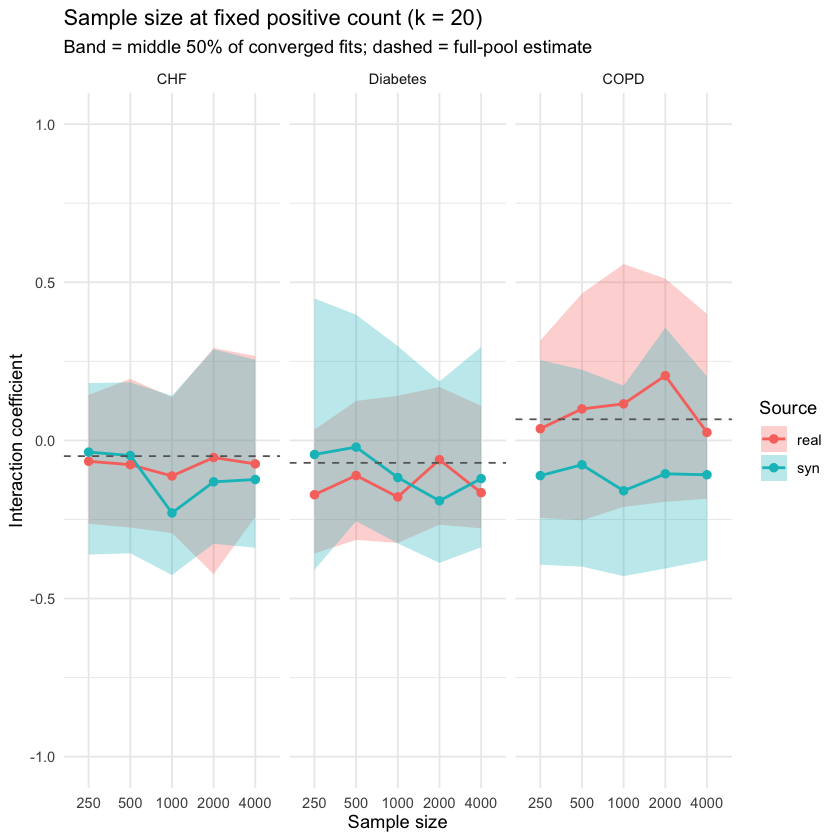
\includegraphics[width=0.55\textwidth]{../figures/size_ribbon.png}
    \caption{Comorbidity $\times$ creatinine with the positive count held
    at 20. Band = middle 50\% of converged fits, dashed line =
    $\hat\beta_{\text{full}}$. In the COPD panel the synthetic median sits
    below the reference at every $n$ and the real median above it.}
    \label{fig:size}
\end{figure}

Width is not the only thing sample size fails to fix. COPD is the one
comorbidity whose interaction is positive, $+0.0668$, and Experiment 1
recovers that sign once the count passes 20. Holding the count at 20 does
not: the synthetic median is negative at all five sample sizes, from
$-0.077$ to $-0.159$, matching the $-0.177$ Experiment 1 recorded at the
same count. Sixteen times the data leaves the sign where twenty positives
put it.

The size effect itself cannot be resolved from noise. The configuration
$k = 20$, $n = 500$ appears in both experiments and so is measured twice
under independent seeds; the readings differ by 13\%, 10\% and 0.3\%, the
same order as the variation across $n$.

\subsection{Tree Diagnosis: The Diagnostic Needs a Null}

\subsubsection*{Count sweep}

What looks like recovery is class balance, not signal. Read without a
control the diagnostic rises from 0 at $k = 5$ to 0.26--0.40 at
$k = 250$, but the permutation null rises with it, from 0.00 to as high as
0.32 (Table~\ref{tab:tree}). What grows alongside the count is the balance
of the column itself, from 1\% positive at $k = 5$ to 50\% at $k = 250$,
and a balanced binary variable is structurally easy to split on whether or
not it carries signal \cite{strobl2007}. Any diagnostic of this form
requires permutation calibration before it can be read.

\begin{table}[H]
\centering
\begin{tabular}{lcccccc}
\toprule
& \multicolumn{2}{c}{CHF} & \multicolumn{2}{c}{Diabetes} & \multicolumn{2}{c}{COPD} \\
\cmidrule(lr){2-3}\cmidrule(lr){4-5}\cmidrule(lr){6-7}
$k$ & Observed & Null & Observed & Null & Observed & Null \\
\midrule
5   & 0.00 & 0.00 & 0.00 & 0.00 & 0.01 & 0.00 \\
10  & 0.04 & 0.01 & 0.00 & 0.01 & 0.04 & 0.01 \\
20  & 0.08 & 0.01 & 0.02 & 0.04 & 0.09 & 0.05 \\
40  & 0.21 & 0.07 & 0.15 & 0.08 & 0.16 & 0.07 \\
80  & 0.21 & 0.23 & 0.27 & 0.15 & 0.30 & 0.19 \\
150 & 0.28 & 0.28 & 0.28 & 0.32 & 0.28 & 0.21 \\
250 & 0.27 & 0.30 & 0.40 & 0.20 & 0.26 & 0.27 \\
\bottomrule
\end{tabular}
\caption{Proportion of replicates in which CART selects the
comorbidity as a split, against its permutation null.}
\label{tab:tree}
\end{table}

Cell by cell the diagnostic is underpowered. Paired tests over the 100
replicates clear $p < 0.01$ in two of the 21 cells, CHF at $k = 40$
($p = 0.004$) and Diabetes at $k = 250$ ($p = 0.002$), and only the latter
survives a Bonferroni correction; both sit isolated among non-significant
neighbours. Pooled over the grid the real column does beat the shuffled
one, 249 discordant replicates to 164, but the margin is thin because the
null has risen to meet it.

\subsubsection*{Size sweep}

Holding the count at 20 runs class balance the other way, from 8\%
positive at $n = 250$ to 0.5\% at $n = 4000$, and the null falls with it,
ending between 0.00 and 0.03 (Table~\ref{tab:treesize}). The null
therefore tracks the balance of the column and nothing else, in a range
the count sweep never reached. The observed rate does not follow it down,
staying between 0.04 and 0.14 at every size, where the count sweep left it
at $k = 20$.

\begin{table}[H]
\centering
\begin{tabular}{rrcccccc}
\toprule
& & \multicolumn{2}{c}{CHF} & \multicolumn{2}{c}{Diabetes} & \multicolumn{2}{c}{COPD} \\
\cmidrule(lr){3-4}\cmidrule(lr){5-6}\cmidrule(lr){7-8}
$n$ & Prevalence & Observed & Null & Observed & Null & Observed & Null \\
\midrule
250  & 8.0\% & 0.05 & 0.03 & 0.07 & 0.02 & 0.06 & 0.08 \\
500  & 4.0\% & 0.04 & 0.02 & 0.08 & 0.04 & 0.06 & 0.01 \\
1000 & 2.0\% & 0.14 & 0.02 & 0.07 & 0.02 & 0.08 & 0.04 \\
2000 & 1.0\% & 0.06 & 0.01 & 0.12 & 0.02 & 0.06 & 0.02 \\
4000 & 0.5\% & 0.07 & 0.00 & 0.09 & 0.01 & 0.04 & 0.03 \\
\bottomrule
\end{tabular}
\caption{CART's use of the comorbidity against its permutation null, with
the positive count held at 20.}
\label{tab:treesize}
\end{table}

With the null near zero the signal becomes legible. Pooled over this grid
the real column wins 104 discordant replicates to 32, and 14 of the 15
cells point the same way, against 249 to 164 in the count sweep. Per cell
the tests stay underpowered, only CHF at $n = 1000$ surviving a Bonferroni
correction over 15 comparisons, but the direction is no longer in doubt:
the diagnostic is readable where its null is near zero, which on this data
means low prevalence.

Neither sweep implicates CART on its own. A GLM fitted to the same
subsamples detects the comorbidity in 2--16\% of replicates in every cell
of both sweeps, against the 6--8\% predicted by rescaling the full-pool
standard errors to $n = 500$, and it does no better on real labels than on
shuffled ones: over the size sweep
the observed rate averages 9.1\% and the permuted 9.5\%, with no trend in
$n$. Both methods are blind at these sizes; CART is the one that fails
visibly, by declining to spend a split.

% -------------------------------------------------------
\section{Discussion}

\paragraph{Two failure modes, not one.}
Reporting the failure rates separately from the spread changed the reading
of this data more than any other decision. Mixing them inflates apparent
instability at low counts, since divergent fits push the quantiles
outward, and it hides the sharpest result in the study, the common
threshold at $k = 80$.

\paragraph{A privacy-fidelity tension.}
CART's reluctance to isolate a subgroup with few supporting cases is not
simply a limitation to work around. A tree willing to carve out a node of
five patients would also be more likely to overfit to, and risk
re-identifying, those individuals, and that same reluctance is what leaves
the stratum missing from the synthetic table in the inestimable cases at
$k = 5$. The tension is a property of the method rather than an
implementation defect, though only its fidelity side is measured here.

\paragraph{The design, not the generator.}
A 500-row subsample carries 6--8\% power against these interactions, and
the GLM arm returned 6.7--10.1\%. Theory and experiment agreeing on a
null result is what rules out a defect in the pipeline and locates the
failure in the design rather than in the generator.

\paragraph{Limitations.}
The diagnostic tree is a proxy for the generator: three predictors rather
than the full feature set \texttt{synthpop} synthesizes jointly, matched
on control parameters but not on its sequential visit order, and counting
the comorbidity as used wherever it appears rather than requiring it
beneath a creatinine split. All three are permissive, which makes non-selection the
more reliable of the two outcomes. Monte Carlo error at $M = 100$ reaches 13\% on
interquartile widths, and the paired tree tests turn on at most 40
discordant replicates per cell in the count sweep and 14 in the size
sweep, so a cell that
misses significance is not evidence that nothing is there. One continuous variable and one outcome were
examined, Renal Failure and Hypertension were screened but not analyzed,
and all results come from a single MIMIC-IV snapshot.

% -------------------------------------------------------
\section{Conclusion}

The positive count governs every quantity measured here, and sample size
governs none of them. Divergence falls to zero at a count of eighty for
all three comorbidities and both data sources; interquartile width falls
by 42--66\% over a matched increase in the count; CART's use of the
comorbidity is flat across a sixteen-fold change in $n$; and a logistic
fit to the same subsamples shows no consistent separation from its
permutation null under either lever. Four readings, two of them from data the synthesizer
never touched. In that narrow sense the finding from Bayesian logistic
regression does extend to CART-based synthesis.

The wider claim does not survive contact with clinical effect sizes. At
practical subsample sizes neither arm recovers the MIMIC-IV interactions:
even the narrowest cell spans nearly four times the quantity being
estimated, and with the count held at 20 the COPD synthetic median
carries the wrong sign at every sample size tested. Where the two can be compared, the synthetic
side is worse on both failure and spread.

For synthetic data evaluation, two things follow: establish
that the target effect is estimable in the source data before attributing
a discrepancy to the generator, and calibrate any variable-selection
diagnostic against a permutation null, since its null moves with class
balance from zero to 0.32 across the range tested here.

% -------------------------------------------------------
{\footnotesize
\begin{thebibliography}{9}

\bibitem{heinze2002}
Heinze, G., \& Schemper, M. (2002).
A solution to the problem of separation in logistic regression.
\textit{Statistics in Medicine}, 21(16), 2409--2419.

\bibitem{nowok2016}
Nowok, B., Raab, G.M., \& Dibben, C. (2016).
\texttt{synthpop}: Bespoke creation of synthetic data in R.
\textit{Journal of Statistical Software}, 74(11), 1--26.

\bibitem{johnson2023}
Johnson, A.E.W., Bulgarelli, L., Shen, L., et al. (2023).
MIMIC-IV, a freely accessible electronic health record dataset.
\textit{Scientific Data}, 10, 1.

\bibitem{strobl2007}
Strobl, C., Boulesteix, A.-L., Zeileis, A., \& Hothorn, T. (2007).
Bias in random forest variable importance measures.
\textit{BMC Bioinformatics}, 8, 25.

\end{thebibliography}
}

\end{document}
